%% Direttive TeXworks:
% !TeX root = ../report.tex
% !TEX encoding = UTF-8 Unicode
% !TEX program = arara
% !TEX TS-program = arara
% !TeX spellcheck = it-IT

% arara: pdflatex: { synctex: yes, shell: yes }
% arara: pdflatex: { synctex: yes, shell: yes }

Essendo lo Sprint iniziale, è stata realizzata un'attenta analisi di tutti i requisiti forniti dal committente
con uno sguardo generale su tutto il sistema, in modo da poter chiarire con quest'ultimo eventuali incomprensioni.

L'obiettivo di questo primo Sprint è individuare struttura e interazioni di massima del sistema; in particolare:
\begin{itemize}
  \item
    con l'analisi dei requisiti si vuole far emergere i componenti del sistema del committente;
  \item
    con l'analisi del problema si vuole identificare eventuali ulteriori componenti di interesse per la futura progettazione.
\end{itemize}

Una volta formalizzata un prima analisi dei requisiti generale, reperibile in questo documento alla \Cref{sec:req_analysis},
il passo successivo è individuare i requisiti prioritari da realizzare in questo primo Sprint, in modo da poterli analizzare nel dettaglio.

\subsection{Analisi dei requisiti}\labelssec{sp1:req_analysis}

Dopo aver delineato tutti i requisiti base, si è scelto di approfondire quelli maggiormente fondanti e di valore per il prodotto.

% TODO

\begin{description}
  \item[\requirementref{R-startExplore}]
    tramite una console grafica l'utente dovrà poter inviare un comando di inizio esplorazione, il comando dovrà essere ricevuto dal robot, il quale dovrà dare inizio alla fase di esplorazione se il requisito successivo è verificato.
  \item[\requirementref{R-Explore}]
    l'esplorazione per questo sprint iniziale consisterà in una serie di mosse dummy, in modo da permettere all'utente di vedere il robot muoversi.
  \item[\requirementref{R-tempOk}]
    l'esplorazione dovrà partire soltanto se la temperatura è inferiore ad una certa soglia. Da requisiti iniziali non è chiaro se il robot debba essere reattivo a cambi della temperatura durante la fase di esplorazione, inoltre non è specificato quale componente debba occuparsi sia del sensing che del checking della temperatura. Ci premureremo di chiarire questi aspetti con il committente.
  \item[\requirementref{R-stopExplore}]
    in seguito ad un comando dell'utente l'esplorazione dovrà essere interrotta ed il robot rimarrà in attesa di sapere dall'utente se deve tornare a casa oppure proseguire l'esplorazione appena interrotta. Non è chiaro cosa debba fare il robot se non gli vengono fornite altre istruzioni.
  \item[\requirementref{R-continueExplore}]
    se l'utente ha inviato il comando per riprendere l'esplorazione il robot deve riprenderla.
  \item[\requirementref{R-backHome}]
    se invece l'utente ha deciso che il robot debba tornare alla sua base, il robot deve farlo. Specifichiamo però che in questo primo sprint non essendo stato ancora introdotto il concetto di mappa, il ritorno a casa sarà soltanto simulato, tuttavia il robot si troverà in uno stato in cui potrà iniziare una nuova esplorazione.
\end{description}

% TODO

Il prodotto dell'analisi dei requisiti deve essere una prima versione dell'architettura logica, che modelli e rappresenti formalmente i requisiti del sistema.

\subsection{Metamodello e QA}\labelssec{qa}

Per rappresentare in maniera formale l'architettura logica, si è scelto di utilizzare il meta-linguaggio QA, nella sua versione 1.5.13.2.
Questo linguaggio è stato messo a disposizione dalla software house e permette di superare le limitazioni intrinseche della modellazione UML
(principalmente object-oriented e con notevoli limitazioni nel distribuito).

\begin{figure}[htbp]
  \centering
  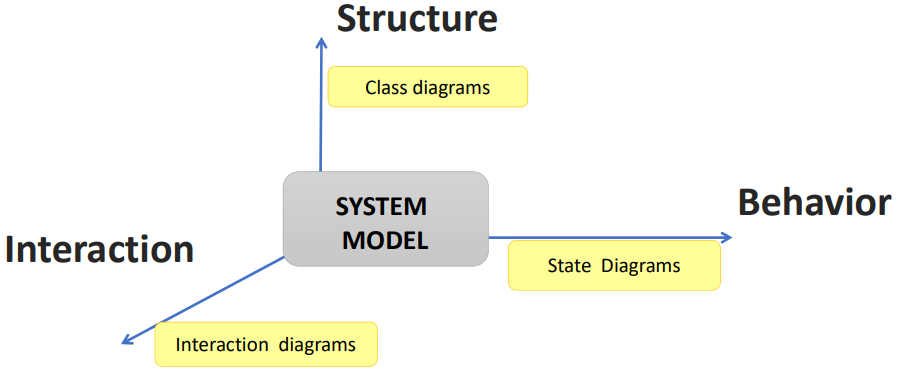
\includegraphics[width=0.75\textwidth]{res/logicalArchitecture.png}%
  \label{fig:logicalArchitecture}
\end{figure}

Il linguaggio QA è adatto per costruire modelli eseguibili di sistemi software e permette di generare rappresentazioni grafiche del sistema,
permettendo di facilitare la comprensione di \textbf{struttura}, \textbf{interazione} e \textbf{comportamento} dello stesso.

\subsection{Architettura logica}\labelssec{sp1:arch_logica_req}

Partendo con un approccio top-down, abbiamo innanzi tutto riconosciuto 3 componenti principali:

\begin{figure}[htbp]
  \centering
  \includegv[width=0.8\textwidth]{res/sprint1/requirements/console}%
  \caption{Console}%
  \label{fig:sp1:console}
\end{figure}

\begin{figure}[htbp]
  \centering
  \includegv[width=0.8\textwidth]{res/sprint1/requirements/robotdiscovery}%
  \caption{Robot Discovery}%
  \label{fig:sp1:robotdiscovery}
\end{figure}

\begin{figure}[htbp]
  \centering
  \includegv[width=0.8\textwidth]{res/sprint1/requirements/robotretrieval}%
  \caption{Robot Retrieval}%
  \label{fig:sp1:robotretrieval}
\end{figure}

Analizzando i tipi di interazioni, abbiamo deciso che queste ultime funzionano come seguono:

\begin{itemize}
  \item
    Il robot invia informazioni sullo stato alla console tramite l'invio di messaggi di tipo \textbf{fire-and-forget}
    (\texttt{dispatch} nel meta-linguaggio QA).

    Essendo il tipo di interazione \textit{uno-ad-uno}, abbiamo ritenuto appropriato utilizzare come metodo di interazione lo scambio di messaggi;
    tra l'altro questo conferisce anche una maggiore sicurezza al nostro sistema.

  \item
    La console invia istruzioni ai robot anch'essa tramite l'invio di messaggi;
    le ragioni sono analoghe al caso precedente,
    e a maggior ragione è evidente come siamo interessati che vi sia uno e soltanto un destinatario.

\end{itemize}

\subsection{Rappresentazione formale}\labelssec{sp1:rapp_formale}

\lstinputlisting[language=qa]{res/sprint1/requirements/robot.qa}

\subsection{Analisi del problema}\labelssec{sp1:prob_analysis}

Durante la fase di analisi del problema abbiamo deciso di dividere il robot discovery in due componenti principali:

Durante la fase di analisi del problema abbiamo deciso di dividere il \textbf{robot discovery} in due componenti principali:

\begin{itemize}
  \item uno che conterrà la business logic (\textbf{robot-mind}).
  \item uno che lavorerà come adattatore per i robot in ambiente virtuale o fisico (\textbf{robot-adapter}).
\end{itemize}

Inoltre abbiamo aggiunto un componente che si occupa di valutare se le condizioni per il funzionamento del robot siano favorevoli o meno e di informare la \textbf{robot-mind}.

Durante l'esplorazione il \textbf{robot discovery} ha anche il compito di costruire una \textbf{mappa} dell'ambiente che potrà essere condivisa;
in questo modo il \textbf{robot retrieval} può elaborare il percorso per raggiungere la bomba all'inizio del suo lavoro.

\subsubsection{World observer}\labelsssec{sp1:world_observer}

Dato che le informazioni ambientali vengono generate esternamente sia al robot che alla console,
abbiamo ritenuto approriato istruire un nuovo componente nel sistema che si occupi di osservare le variazioni delle condizioni ambientali
e che vada a valutarle per decidere se queste sono favorevoli o meno al corretto funzionamento del robot;
una volta valutate tali condizioni, il componente emette un evento tramite il quale informa il resto del sistema.

\subsubsection{Robot Adapter e Robot Mind}\labelsssec{sp1:mind_adapter}

Abbiamo ritenuto opportuno separare la logica di funzionamento del robot dal componente che si occupa di eseguire le istruzioni per vari motivi,
tra cui ottenere una maggiore separazione tra un componente chiave contenente la \textbf{business logic} che è il core del nostro sistema (\textbf{robot-mind}) ed un mero esecutore di comandi (\textbf{robot-adapter}).
Tra l'altro questo ci garantisce un maggior livello di \textbf{technology independency}, \textbf{riusabilità} e \textbf{tracciabilità} nel nostro sistema.

Il robot-adapter altro non è che un \textbf{driver} che esegue i comandi ricevuti dalla \textbf{mind} nel mondo fisico o in quello virtuale (o in entrambi) e non deve sapere nulla della logica di funzionamento del sistema.

